\begin{titlepage}

\centering

\begin{tikzpicture}

%\node[opacity=0.3,inner sep=0pt,remember picture,overlay] at (4.5,-0.5){\includegraphics[width= 0.8 \textwidth]{Figures/0. General/Logo Bild.jpg}};

\node[inner sep=0pt] (logo) at (0,0)
   {
\includegraphics[width=.5\textwidth]{Figures/0. General/02_uio_full_logo_eng_pos.jpg}};
    
\node[text width = 0.5\textwidth, right = of logo](title){\sffamily\huge\reporttitle};

\node[text width = 0.5\textwidth, yshift = 0.75cm, below = of title](subtitle){\sffamily\Large \reportsubtitle};

\gettikzxy{(subtitle.south)}{\sffamily\subtitlex}{\subtitley}
\gettikzxy{(title.north)}{\titlex}{\titley}
\draw[line width=1mm, Tue-red]($(logo.east)!0.5!(title.west)$) +(0,\subtitley) -- +(0,\titley);

\end{tikzpicture}
\vspace{3cm}

\sffamily\groupnumber

\begin{table}[H]
\centering
\sffamily
\large
\begin{tabu} to 0.8\linewidth {c}
\textbf{\LARGE{Involved students}} \\
%\textbf{\LARGE{Student ID}}\\
\hline

\sffamily\reportauthors

\end{tabu}

\end{table}

\sffamily \grouptutor


\\ \ \\ \ \\
\begin{flushright}
\small{Picture by \href{https://flickr.com/photos/dalbera/4840429336/}{Annie Dalbéra}. \href{https://creativecommons.org/licenses/by/2.0/deed.de}{CC BY 2.0}}
\end{flushright}
\tikz[remember picture,overlay]\node[anchor=south,inner sep=0pt] at (current page.south) {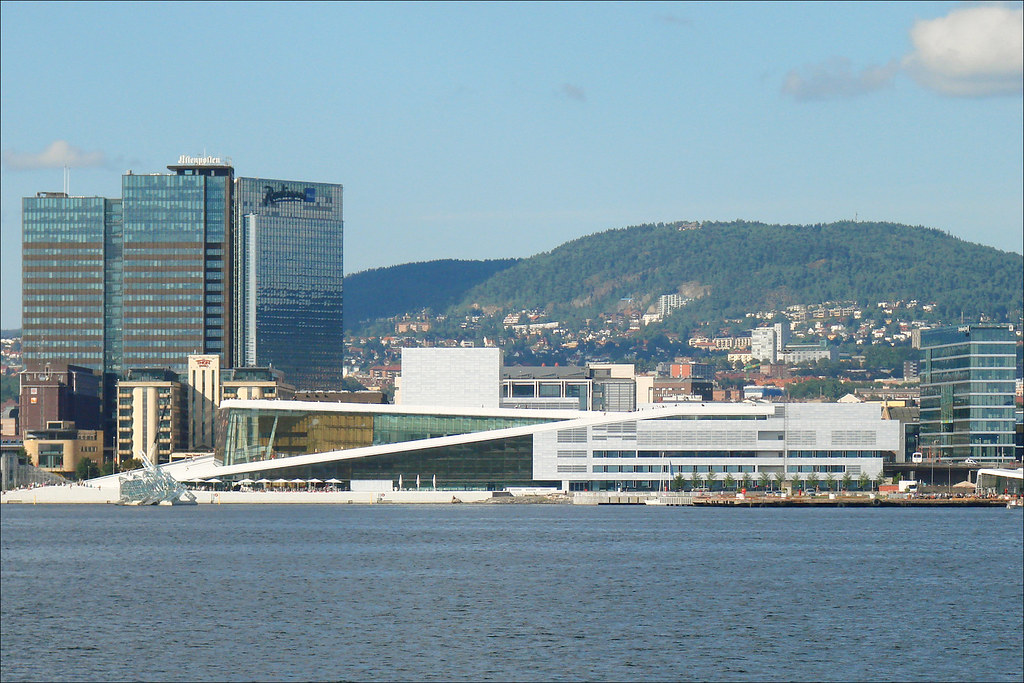
\includegraphics[width=\paperwidth, height=13cm]{Figures/0. General/Oslo image.jpg}};

\mbox{}
\vfill
\sffamily \Large \textcolor{white}{\placeanddate } \\
\end{titlepage}








